%%%%%%%%%%%%%%%%%  Debut du fichier Latex  %%%%%%%%%%%%%%%%%%%%%%%%%%%%%%
\documentclass[a4paper,12pt,onecolumn]{article}

%%% Pour un texte en francais

%%\usepackage[applemac]{inputenc}
%\usepackage[francais]{babel}
	         % encodage des lettres accentuees
\usepackage[T1]{fontenc}
\usepackage[utf8]{inputenc}          % encodage des lettres accentuees
%\usepackage{graphicx}
%%\usepackage{graphicx} \def\BIB{}
\usepackage[paper=a4paper,textwidth=140mm,left=2.8cm,right=2.8cm,top=3cm,bottom=3cm]{geometry}
\usepackage{multicol}
\usepackage{graphicx,wrapfig,lipsum} 
%\def\BIB{}
\usepackage[font=footnotesize]{caption}
\usepackage{subcaption}
\usepackage[pdftex]{hyperref}
\usepackage{natbib}
\usepackage{url}
\usepackage{xspace}
\usepackage{perpage} %the perpage package
\MakePerPage{footnote} %the perpage package command
\hypersetup{
    colorlinks,%
    citecolor=black,%
    filecolor=black,%
    linkcolor=black,%
    urlcolor=blue     % can put red here to visualize the links
}
\usepackage{changepage}
\usepackage{atbegshi}
% to delete the first page which appears when I use adjustwidth
\AtBeginDocument{\AtBeginShipoutNext{\AtBeginShipoutDiscard}} 

\DeclareUnicodeCharacter{00A0}{ }

%%% Quelques raccourcis pour la mise en page
\newcommand{\remarque}[1]{{\small \it #1}}
\newcommand{\rubrique}{\bigskip \noindent $\bullet$ }

\newcommand{\ignore}[1]{}

\renewcommand*\rmdefault{iwona}

\pagenumbering{gobble}

\newcommand{\sgx}{SgXB\xspace}
\newcommand{\sfxt}{\textsc{sfxt}}
\newcommand{\sg}{Sg\xspace}
\newcommand{\co}{CO\xspace}
\newcommand*{\hmxb}{HMXB\@\xspace}
\newcommand*{\rlof}{RLOF\@\xspace}
\newcommand*{\ns}{NS\@\xspace}
\newcommand*{\bh}{BH\@\xspace}
\newcommand*{\eg}{e.g.\@\xspace}
\newcommand*{\ie}{i.e.\@\xspace}
\newcommand*{\aka}{a.k.a. \@\xspace}

%\bibliographystyle{abbrvnat}
%\setcitestyle{authoryear,open={((},close={))}}

%\renewcommand{\thefootnote}{\roman{footnote}}

% -------------------------------------------------
\newcommand{\horrule}[1]{\rule{\linewidth}{#1}} % Create horizontal rule command with 1 argument of height

\title{	
\vspace*{-2cm}
\normalfont \tiny 
%\textsc{Paris Diderot} \\ [25pt] % Your university, school and/or department name(s)
\horrule{0.5pt} \\[0.4cm] % Thin top horizontal rule
\huge Research project \\ \vspace*{0.5cm} \textbf{Accretion onto stellar remnants in binaries} \\ % The assignment title
\horrule{2pt} \\[0.5cm] % Thick bottom horizontal rule
}
\author{El Mellah Ileyk} % Your name
\date{\tiny }%\normalsize\today} % Today's date or a custom date
% -------------------------------------------------

%\makeatletter
%\def\@xfootnote[#1]{%
%  \protected@xdef\@thefnmark{#1}%
%  \@footnotemark\@footnotetext}
%\makeatother

\begin{document}

%\bibpunct{[}{]}{;}{n}{,}{,}

%%%%%%%%%%%%%%%%%%%%%%%%%  PREMIERE PAGE %%%%%%%%%%%%%%%%%%%%%%%%%%%%%%
%%% DANS CETTE PAGE, ON REMPLACE LES INDICATIONS ENTRE CROCHETS [...]
%%% PAR LES INFORMATIONS DEMANDEES
%%%%%%%%%%%%%%%%%%%%%%%%%%%%%%%%%%%%%%%%%%%%%%%%%%%%%%%%%%%%%%%%%%%%%%%

\begin{adjustwidth}{-0.4cm}{-0.4cm}
\maketitle
\end{adjustwidth} 

\thispagestyle{empty}

In the past year, I coupled numerical simulations centered on the accretor to results concerning the overdensities (or clumps) formed in the line-driven wind of hot stars due to internal shocks. I characterized the impact of these clumps on the time variability of the mass accretion rate inflowing within a sphere of a few hundreds times the size of the compact object and centered on it. The latter corresponds approximately to the dimension of the neutron star (\ns) magnetosphere, the region where magnetic effects can no longer be discarded. We now need to investigate other sources of time variability than the clumps to interpret the observations :
\begin{itemize}
\item the presence of a transient disc-like structure around the accretor could lead to specific disc instabilities (\eg the magneto-rotational instability).
\item magnetic and centrifugal gatings at the edge of the NS magnetosphere are expected to contribute to break up the accreted flow, along with thermodynamical considerations which modulate the entry within the NS magnetosphere.
\item the X-ray ionizing feedback from the immediate vicinity of the accretor alters the dynamics of the wind at the orbital scale.
\end{itemize}
These 3 trails form the backbone of my research project in the following years. If it is mostly aimed at Supergiant X-ray binaries (\sgx) and Supergiant Fast X-ray Transients (SFXT), it has also ramifications to similar systems such as Cataclysmic Variables (CV), low mass X-ray binaries or Be X-ray binaries. Thanks to the suited numerical framework I contributed to develop over the last years, we can aspire to obtain, by the end of the next decade, a consistent overview of the mass transfer process, from the Dantean stellar surface down to the magnetic vicinity of a NS, if not the relativistic surroundings of a black hole. Current missions (\eg XMM-Newton, Chandra and Integral) provide us with the guiding constrains of our numerical investigations, while future ones (\eg SVOM, LOFT and Athena) will bring unprecedented observations which will confront theoretical expectations even further.

\newgeometry{left=2.1cm,right=2.1cm,top=2.8cm,bottom=2.8cm}
\newpage

\subsubsection*{Wind-capture discs}

\begin{wrapfigure}{r}{7.2cm}
\vspace*{-1.5cm}
\hspace*{0.1cm}
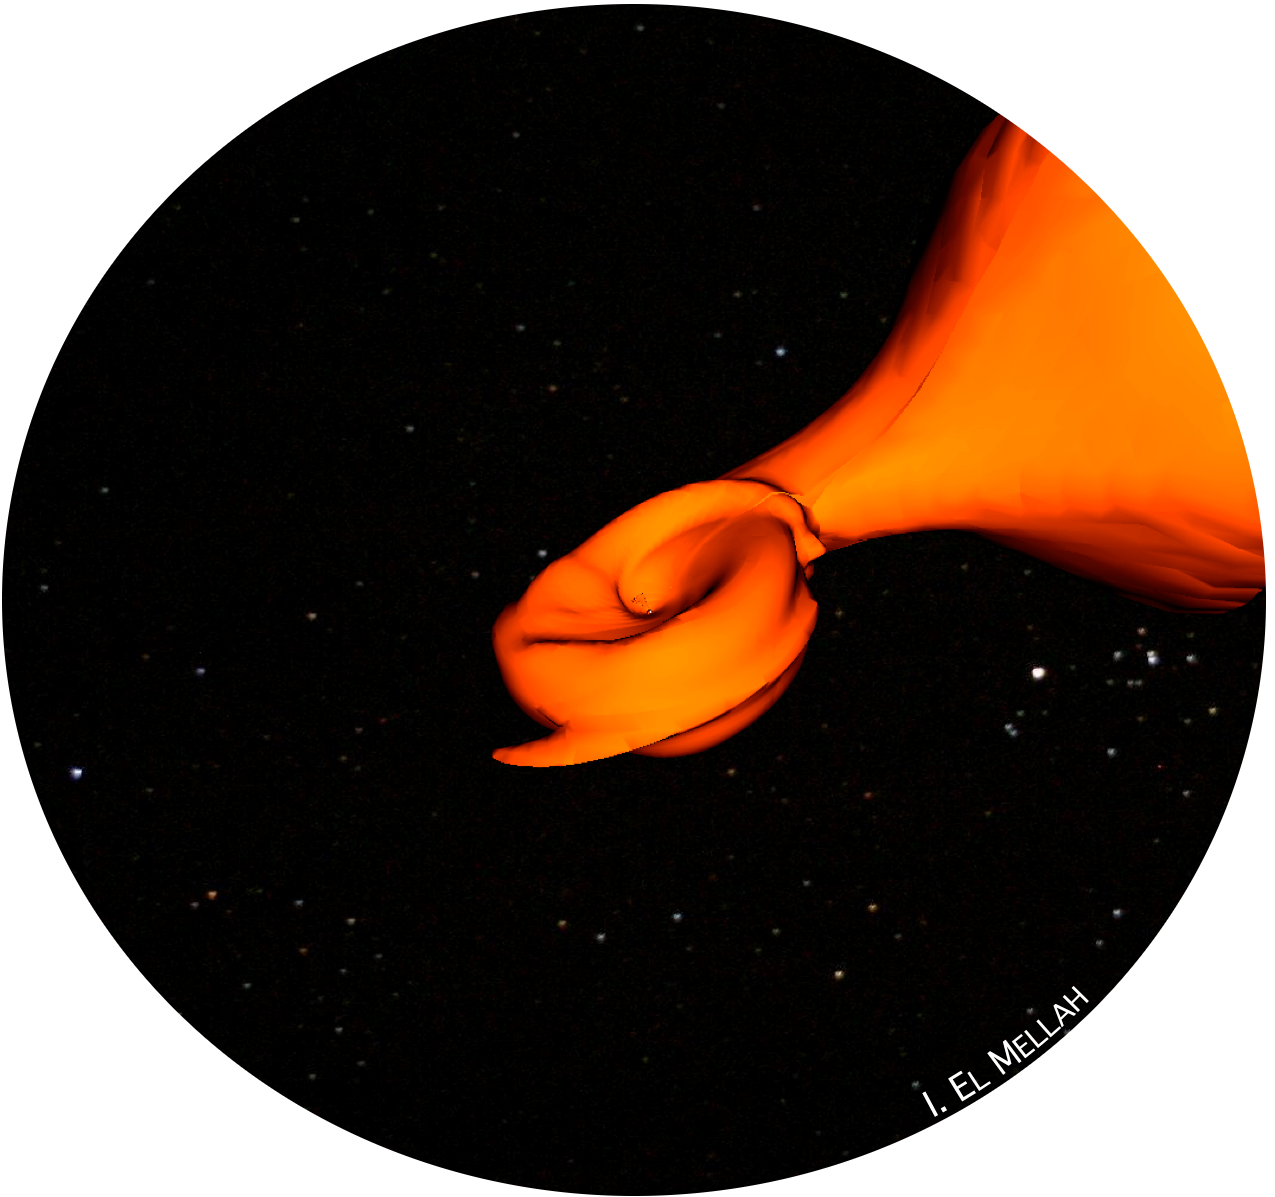
\includegraphics[height=7.1cm]{Figures/RLOF.png}
\caption{Isodensity surface of a 3D flow from a \rlof star (upper right) to an accretor, 1,000 times smaller than the orbital separation between the two bodies.}
\label{fig:bow2.5d}
\end{wrapfigure} 

The first step of this research project addresses the capacity of the accreted flow to form a disc, depending on the speed of the flow compared to the orbital speed. In the low speed-limit, a Roche lobe overflowing (\rlof) star pours matter at the first Lagrangian point directly into the Roche lobe of the accretor (see Figure\,\ref{fig:bow2.5d}). The flow winds up around the accretor and forms a large permanent disc. In the high-speed limit, long thought to be valid for \sgx, the line-driven wind coming from a high mass donor star carries little angular momentum : the flow structure is described by the Bondi-Hoyle-Lyttleton solution and no disc is expected. However, \cite{Mohamed2011} laid the foundations for a treatment of the intermediate case or \textit{wind-RLOF}. In \cite{ElMellah2016a}, I adapted it for \sgx. Recent observational and numerical results on the wind speed in the classic \sgx Vela X-1 suggest that neither of the 2 aforementioned asymptotic cases apply \citep{Gimenez-Garcia2016,Sander2017} and a wind-RLOF approach is required. I plan to study this case to identify the conditions of formation of wind-captured discs (see Figure\,\ref{fig:wind-RLOF}). Discs are known to be fruitful landscapes for a plethora of instabilities which might partly contribute to the time variability in some \sgx.\\ \\

\begin{wrapfigure}{l}{7.2cm}
\vspace*{-0.5cm}
\hspace*{0.1cm}
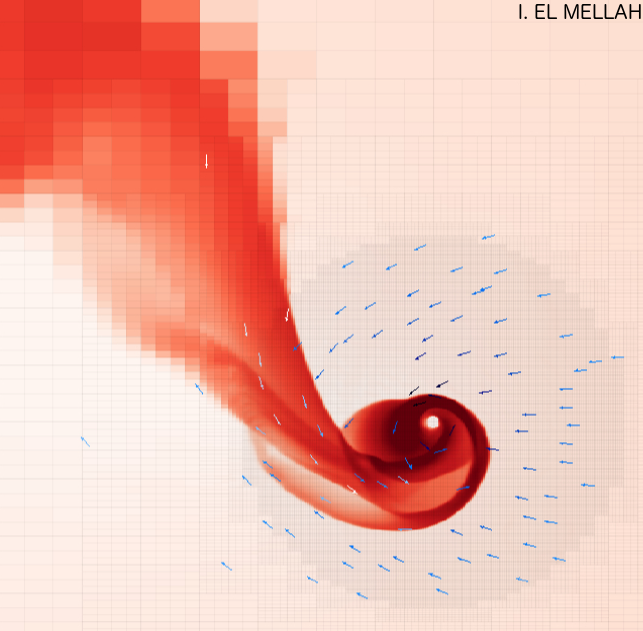
\includegraphics[height=7.1cm]{Figures/wind-RLOF.png}
\caption{Density and velocity map of a slow wind (coming from the right) being accreted onto a compact object. The detached bow shock becomes a disc-like structure.}
\label{fig:wind-RLOF}
\end{wrapfigure} 

\indent This problem would make the most of ray-tracing tools such as \texttt{GYOTO} \citep{Vincent2011} whose main developers work at the LUTh (Eric Gourgoulhon) or at the neighboring LESIA (Fr\'ed\'eric Vincent, Thibaut Pomard \& Guy Perrin). Indeed, for a \sgx hosting a black hole such as Cygnus X-1, progresses on the structure of the disc and its environment would bring, once processed with \texttt{GYOTO}, new insights on the photometric and spectroscopic properties. Also, low angular momentum accretion onto a compact object is a subject of prime importance for Sagittarius A* which is observed with the GRAVITY instrument managed, among others, by the LESIA.

\clearpage

%\newgeometry{left=2cm,right=2cm,top=2.6cm,bottom=2.6cm}

\newpage

%To guarantee that we work with physically consistent accretion discs, I am now performing numerical simulations of RLOF configurations where the expanded atmosphere of the donor star is channeled into the Roche lobe of the accretor through the first Lagrangian point. This model includes a proxy on viscosity, similar to the one introduced by \cite{Shakura1973}, and energy losses through radiative cooling. The former stands for the turbulent viscosity associated to the magnetic rotational instability \citep{Balbus1991}. Together with spiral shocks, they participate to the evacuation of angular momentum which makes the accretion possible. The ballistic solution is then superseded by the actual formation of a disc around the accretor. Since the plasma largely exceeds 10,000K during the accretion process, a significant fraction of the elements is ionized. We make use of the SPEX cooling tables for solar abundances to compute the cooling function \citep{VanMarle2011}, which yields cooling rates large enough to impact the thickness of the flow. However, the numerically convenient optically thin assumption we currently make breaks up in the disc and must be complemented with a flux-limited diffusion method I plan to implement in \texttt{MPI-AMRVAC}. These improvements could first lead to insights concerning the origin of negative superhumps in cataclysmic variables \citep[CV, ][]{Murray1998}. Replacing the inner accretor with a \bh or a lowly magnetized NS, the wrapping of the disc could also be studied and numerical results obtained in the context of Smooth Particle Hydrodynamics simulations could be confronted \citep{Foulkes2006}. If the disc turns out to be misaligned with the orbital plane, it could have a serious impact on jet-launching conditions since a misalignement with the \bh spin is likely to induce a precession of the jets \cite{Liska2017}.

\subsubsection*{The NS magnetosphere}

\begin{wrapfigure}[13]{r}{5.2cm}
\vspace*{-1cm}
\hspace*{0.1cm}
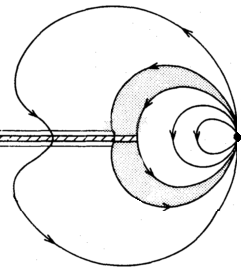
\includegraphics[height=5.1cm]{Figures/ghosh_lamb.png}
\caption{Truncation of the inner disc by the NS magnetosphere. From \cite{Ghosh1978}.}
\label{fig:ghosh}
\end{wrapfigure} 

The NS in \sgx are strongly magnetized since their young age did not allow for a significant decay of their pristine dipolar field. Within the magnetosphere, magnetically-funneled accretion onto the poles takes place. Yet, the contrast between the size of the NS and the orbital separation makes it challenging to develop a numerical setup suitable for magneto-hydrodynamical problems. To alleviate this obstacle, we started with Zakaria Meliani (LUTh) to study a family of binaries where the accretor is one hundred times larger and where the orbital separation is ten times smaller : cataclysmic variables (CV). These systems still retain the main qualitative ingredients as \sgx while being much more computationally affordable. In intermediate polars, a sub-class of CV, a RLOF star feeds an accretion disc truncated at its innermost border by the magnetic field of the accreting white dwarf (see Figure\,\ref{fig:ghosh}). The flow is then funneled to the WD poles where it is shocked and heated to high temperatures, emitting copious amounts of light. We are currently implementing a grey cooling method into our code, \texttt{MPI-AMRVAC}, to see the interplay between a physically-motivated stratified disc and the WD magnetic field. Coupled to the adaptive mesh stretched grid I developed during my PhD, this approach could improve our understanding of the WD spinning down. More generally, such a setup will be also used to set constrains on the disc reformation after a nova \citep{Ness2012} : with U Scorpii expected to go off in a couple of years, I started to collaborate with Jan-Uwe Ness (ESAC) to write together an observation proposal by summer 2018.\\
\indent This twofold setup also serves another purpose : diving into the magnetosphere of the accreting NS in \sgx, where the magnetic field is larger. Numerically, we recently implemented and validated a method of magnetic splitting generalized to non-potential fields \citep{Xia2017}. It enables us to handle more accurately the magnetic field evolution, in particular in magnetically-dominated plasmas, and to clean more easily the non-zero divergence. With this new feature available, we want to study how the innermost parts of the wind behave. Depending on how the magnetosphere radius compares with other characteristic length scales such as the accretion and corotation radii, the flow might be halted and cascade later on within the magnetosphere \citep{Bozzo2008}. We can now study this modulation with physical inputs accounting for the variability at the upper scales derived in \cite{ElMellah}. We also want to address the case where the NS magnetospheric radius is much larger, of the order of the accretion radius. How does it alter the shock? 
 	
\subsubsection*{X-ray ionizing feedback}

Eventually, early 2017, I joined a collaboration of X-ray binaries observers and experts of winds of massive stars, a collaboration which became the X-wind team later in the year. Among this team, my role is to connect the information we get from state-of-the-art numerical simulations of line-driven winds of isolated massive stars \citep{Sundqvist2017,Sander2017} to the variability of the X-ray emission and absorbing column density characterized by the observers in \sgx \citep{Grinberg2017}. The next step to perform this connection in a self-consistent way is to evaluate the radiative influence of the X-rays emitted in the immediate vicinity of the accretor on the inflowing wind. Indeed, the efficiency of line-driven acceleration drops when the wind gets excessively ionized \ie as it gets closer from the accretor it feeds. In the continuation of \cite{Blondin1990}, \cite{Manousakis2015c} performed 2D simulations where they accounted for this effect but prescribed an a priori fixed X-ray luminosity. We aim at dynamically computing this X-ray luminosity from the mass accretion rate at the inner border of the large scale contrast simulation space introduced in \cite{ElMellah}. The X-wind collaboration workshop of October 2018 in Santander will be the occasion to confront these results to new observations, while our monthly telecons allow us to keep track of the intermediate steps performed by each of the 25 members or so.\\

Since the end of my PhD, I have built up multiple collaborations to embed the numerical tool into the scientific method, as a binder between the theoretical approach, limited by the mathematical tools available, and the observational approach, limited by the instruments at our disposal. Thanks to the high performance computing technologies, Computational Astrophysics has ushered in a particularly exciting period to address a wide range of questions pertaining to accretion, from Active Galactic Nuclei to X-ray binaries and planetary formation. Concomitantly, the multiple confirmed detections of gravitational waves from coalescing compact objects have urged even more the community to evaluate the impact of binarity on the evolutionary tracks of massive stars. To this extent, high mass X-ray binaries represent a decisive stage whose understanding would shed light on many fundamental questions, from the scarcity of intermediate mass black holes to the equation-of-state of matter at supernuclear densities in neutron stars. A position as a researcher at the LUTh, whose members show a shared interest in compact objects and their surroundings, would enable me to carry on this research program and reinforce the connections I built up with the scientific community in France. I would also strengthen the numerical expertise of the LUTh and support the Observatoire de Paris-Meudon in its effort to introduce the next generation of researchers to advanced computational skills.\\


%To conclude, the numerical expertise I have developed in Computational Astrophysics enables me to make the most of the high performance computing technologies available. They have ushered in a particularly exciting period to address a wide range of questions pertaining to accretion in X-ray binaries. To progress on these questions in the following 5 years a tenure track at the University of Amsterdam would offer me, I need to keep connecting with observers and modelers in this field. The research activity of the Anton Pannekoek Institute for Astronomy shows a shared interest in the key-questions of accretion-ejection processes and the neutron star equation-of-state. The former intersects the question of the disc structure we try to address, while the latter would take advantage of more constraining predictions on the properties of the accreted flow. To raise the funds necessary to such a project, I intend to apply to ambitious funding such as the ERC grants. Beyond their autonomous requirements and satisfactions, I also expect my teaching duties to be opportunities to arouse the interest of the students in pursuing in this research domain. Should it be the case, I would gladly mentor them, as I have been mentored on my way to the endlessly mesmerizing field of Astrophysics. 

%\indent More generally, the B field opens the door to a wide range of accretion-ejection mechanisms in the disc itself (Blandford-Payne 82, Casse 04), provided we have a physically-motivated disc thickness profile (see previous section). Transition from jet emitting discs to standard accretion discs (SS75) as a possible explanation for the two states observed in LMXB (Ferreira 06).\\ \\

%\section*{Conclusion}
%
%Bedrock model 
%
%Longer term prospective

\vspace*{-0.1cm}
%\subsubsection*{References}
{\def\section*#1{}
%\newgeometry{left=2cm,right=2cm,top=2.5cm,bottom=2.5cm}
\setlength{\bibsep}{5pt}
\footnotesize
\bibliographystyle{agsm}
\bibliography{/Users/Ileyk/Documents/Bibtex/research_statement_no_url}
}

%\newgeometry{left=2cm,right=2cm,top=2.5cm,bottom=2.5cm}
%\setlength{\bibsep}{5pt}
%\small
%\bibliographystyle{agsm}
%\bibliography{/Users/Ileyk/Documents/Bibtex/research_statement_no_url}

\newpage

\phantom{n}

\end{document}
%%%%%%%%%%%%%%%%%  Fin du fichier Latex  %%%%%%%%%%%%%%%%%%%%%%%%%%%%%%

